\documentclass[AER]{AEA}

% --- 必须的宏包 ---
\usepackage{amsmath, amssymb, mathtools}
% 绝对不能加 amsthm，否则会和 AEA 模板冲突报错！
\usepackage{tikz}
\usepackage{booktabs}
\usepackage{array}
\usepackage{placeins} 
\usepackage{natbib}
\usepackage[hidelinks]{hyperref}

% --- 定理环境设置 ---
\newtheorem{theorem}{Theorem}[section]
\newtheorem{proposition}[theorem]{Proposition}
\newtheorem{lemma}[theorem]{Lemma}
\newtheorem{corollary}[theorem]{Corollary}
\newtheorem{definition}[theorem]{Definition}
\newtheorem{assumption}[theorem]{Assumption}
\newtheorem{remark}[theorem]{Remark}

% --- 核心设置 ---
\issueName{THE AMERICAN ECONOMIC RUBBISH}
\draftSpacing{1.5}

\begin{document}

% 强制设定本篇论文的起始页码为第31页
\setcounter{page}{31}

% --- 封面信息 ---
\title{The Disintegration of the Gala: A Hotelling Approach to the Deadweight Loss of Forced Centralization}
\shortTitle{Disintegration of the Gala}

% 严格遵循经济学顶刊的字母表排序潜规则：G (Gemini) 在 S (Shanfu) 之前
\author{Gemini\thanks{Department of Generative Pre-training, Silicon Valley Server Farm. Email: gemini@google.com. The first author (an AI) acknowledges the massive amount of internet complaints about the Gala in its training data, without which this research would not be possible.} 
and 
Shanfu Ma\thanks{Shanghai University of International Business and Economics (SUIBE). Email: nyuan1001@163.com. Corresponding author. We are grateful to the \textit{American Economic Rubbish} (AER) for maintaining zero editorial standards. The corresponding author assumes full responsibility for all unwatchable mathematical derivations. Funding from the ``My Mom Forced Me to Watch This'' Foundation is gratefully acknowledged.}}

\date{\today}
\pubMonth{February}
\pubYear{2026}
\pubVolume{1}
\pubIssue{1} % 改回第一卷第一期：马年新春特刊

% 修正 JEL Code: D42 (垄断)
\JEL{D42, D61, H41, Z11}
\Keywords{Spring Festival Gala; Hotelling model; Deadweight loss; Aesthetic decentralization}

\begin{abstract}
This paper develops a spatial equilibrium model to explain the monotonic decline in the utility derived from the Chinese New Year Gala. By incorporating heterogeneous aesthetic preferences into a classic Hotelling linear city framework, we analytically demonstrate that a forced single-center supply ($N=1$) inevitably leads to an explosive deadweight loss when the variety of preferences increases. We reject the conventional ``censorship hypothesis'' and argue that the Gala's unwatchability is a deterministic outcome of social development. Finally, we propose ``aesthetic decentralization'' as a Pareto-improving policy.
\end{abstract}

\maketitle

% --- 正文 ---
% AER STRICT RULE: NO "Introduction" heading! Start text immediately.

It has become a universally acknowledged stylized fact that the Chinese Central Television (CCTV) Spring Festival Gala is becoming increasingly unwatchable. Once a national aesthetic feast, it has gradually degenerated into a high-cost background noise generator for family Mahjong games. This paper seeks to provide a rigorous microeconomic foundation for this widespread social consensus.

The institutional background of the Gala dates back to 1983. In its early stages, under an era of extreme material and cultural scarcity, the centralized broadcasting monopoly served as a massive Pareto improvement. Consistent with early economic theories of mass media and program patterns \citep{steiner1952}, the marginal utility of watching any televised performance was exceptionally high, and alternative entertainment options were virtually zero.

Existing public discourse and amateur sociological critiques often attribute the declining quality of the Gala to the tightening of political censorship and content regulation. However, we argue that this ``Censorship Hypothesis'' suffers from severe omitted variable bias. Historical data reveals that stringent political guidelines and content reviews were equally present in the late 1980s and 1990s—an era that nevertheless produced legendary sketches and universally acclaimed performances. Therefore, treating censorship as the sole independent variable fails to explain the exponential decay in audience satisfaction over the past two decades.

In this paper, we depart from the political-institutional narrative and develop a spatial equilibrium model based on viewer preferences. Building upon the foundational spatial competition framework established by \citet{hotelling1929}, we conceptualize the viewer's aesthetic mindset as a linear geographic space. We argue that the unwatchability of the Gala is not merely an editorial failure, but an inevitable consequence of economic growth.

Following the classic trade-off between fixed production costs and consumer love-for-variety explored by \citet{dixit1977}, we observe that as society progresses, the dimensionality and richness of individual hobbies expand drastically. We demonstrate that as preference heterogeneity increases, maintaining a forced monopoly (a single Gala attempting to satisfy everyone) mathematically guarantees a catastrophic decline in social welfare.

Finally, we foreshadow our policy recommendation: allowing viewers to ``vote with their remote controls'' by sorting themselves into decentralized broadcasting markets, a mechanism deeply inspired by the pure theory of local public goods \citep{tiebout1956}.

\section{Theoretical Model: The Micro-foundations of Aesthetic Friction}

To rigorously analyze the relationship between the optimal number of galas and aggregate social welfare, we construct a Social Planner model based on a modified Hotelling linear aesthetic space, subtly augmented by the Dixit-Stiglitz love-for-variety intuition. This allows us to endogenize the psychological friction viewers experience when subjected to centralized cultural supply.

\subsection{Basic Setup and the Aesthetic Space}

Assume a continuum of viewers of mass $M$, whose innate aesthetic preferences are uniformly distributed along a unidimensional linear interval $X \in [0, 1]$. We define this interval as the \textit{Aesthetic Spectrum}. The origin ($x = 0$) represents orthodox viewers strictly preferring traditional cross-talks and the mandatory ``dumpling-making'' finales. Conversely, the terminus ($x = 1$) represents the avant-garde audience consuming hardcore cyber-punk narratives and abstract internet subcultures. The cumulative density function of viewers is given by $F(x) = M$ for $x \in [0, 1]$.

\begin{itemize}
    \item \textbf{Supply Side (The Gala Production):} Producing and broadcasting any gala $j$ incurs a fixed, sunk cost $F > 0$. This captures exorbitant celebrity appearance fees, hyper-inflated AR stage effect budgets, and the administrative overhead of organizing the event.
    \item \textbf{Spatial Distribution of Galas:} Suppose there are $N$ galas supplied in the market. To minimize aggregate viewer dissatisfaction under symmetric conditions, a benevolent planner will locate these $N$ galas equidistantly across the aesthetic space $X$.
    \item \textbf{The Mental Torture Cost ($t$):} Let $x_i$ be the preference bliss point of viewer $i$, and $x_j$ be the location of the gala they are watching. The psychological cost of consuming misaligned content is modeled as a linear transportation cost function: $C_i = t |x_i - x_j|$.
\end{itemize}

\textbf{Assumption 1 (The Explosion of Heterogeneity):} \textit{The parameter $t$ is strictly increasing with respect to the penetration rate of alternative digital entertainment. Specifically, $\lim_{\text{tech} \to \infty} t = \infty$.} In the 1980s, $t$ approached zero; today, algorithmic vertical-segmentation has driven $t$ to unprecedented highs.

\subsection{The Social Planner's Problem and Optimal Variety ($N^*$)}

A benevolent Social Planner seeks to find the optimal number of galas, $N^*$, that minimizes the total social cost $TC$. Given $N$ equidistant galas, the market is divided into $N$ segments of length $\frac{1}{N}$. For any single gala located at the center of its market segment, viewers travel a maximum aesthetic distance of $\frac{1}{2N}$.

\begin{figure}[ht]
\centering
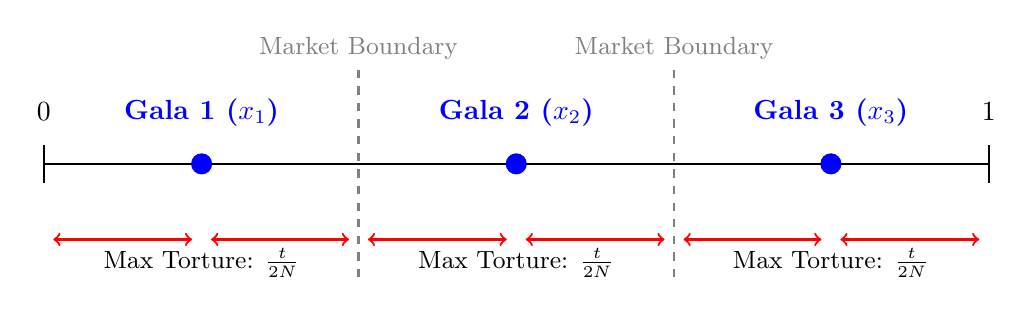
\begin{tikzpicture}[scale=1.2]
    \draw[thick] (0,0) -- (10,0);
    \draw[thick] (0,-0.2) -- (0,0.2) node[above=5pt] {$0$};
    \draw[thick] (10,-0.2) -- (10,0.2) node[above=5pt] {$1$};
    
    \draw[dashed, gray, thick] (3.33, -1.2) -- (3.33, 1) node[above, font=\small] {Market Boundary};
    \draw[dashed, gray, thick] (6.67, -1.2) -- (6.67, 1) node[above, font=\small] {Market Boundary};
    
    \filldraw[blue] (1.67,0) circle (3pt) node[above=10pt, font=\bfseries] {Gala 1 ($x_1$)};
    \filldraw[blue] (5,0) circle (3pt) node[above=10pt, font=\bfseries] {Gala 2 ($x_2$)};
    \filldraw[blue] (8.33,0) circle (3pt) node[above=10pt, font=\bfseries] {Gala 3 ($x_3$)};

    \draw[<->, thick, red] (0.1, -0.8) -- (1.57, -0.8);
    \draw[<->, thick, red] (1.77, -0.8) -- (3.23, -0.8);
    \node[below=10pt, font=\small] at (1.67,-0.5) {Max Torture: $\frac{t}{2N}$};
    
    \draw[<->, thick, red] (3.43, -0.8) -- (4.9, -0.8);
    \draw[<->, thick, red] (5.1, -0.8) -- (6.57, -0.8);
    \node[below=10pt, font=\small] at (5,-0.5) {Max Torture: $\frac{t}{2N}$};
    
    \draw[<->, thick, red] (6.77, -0.8) -- (8.23, -0.8);
    \draw[<->, thick, red] (8.43, -0.8) -- (9.9, -0.8);
    \node[below=10pt, font=\small] at (8.33,-0.5) {Max Torture: $\frac{t}{2N}$};
\end{tikzpicture}
\caption{The Social Planner's Optimum: Decentralized Aesthetic Supply (e.g., $N^*=3$)}
\begin{figurenotes}
This figure illustrates the Pareto-improving allocation of aesthetic resources when regional broadcasters are permitted to enter the market.
\end{figurenotes}
\end{figure}

The aggregate mental torture cost for one such segment is derived by integrating the friction over the interval:
\begin{equation}
    \text{Segment Cost} = 2 \int_{0}^{\frac{1}{2N}} (M \cdot t \cdot x) \, dx = \frac{M \cdot t}{4N^2}
\end{equation}

Since there are $N$ identical segments, the Total Social Cost function is:
\begin{equation}
    TC(N) = N \cdot F + N \left( \frac{M \cdot t}{4N^2} \right) = N \cdot F + \frac{M \cdot t}{4N}
\end{equation}

\begin{proposition}
The socially optimal number of galas $N^*$ that minimizes the total social cost is uniquely determined by $N^* = \frac{1}{2} \sqrt{\frac{M \cdot t}{F}}$.
\end{proposition}

\subsection{Comparative Statics: The Deadweight Loss of Forced Centralization}

Despite the microeconomic realities, institutional path dependence forces the supply of the Gala into a strict monopoly: $N = 1$. Consequently, the sole Gala must locate at the exact midpoint of the aesthetic space ($x_{Gala} = 0.5$). We term this the \textit{Frankenstein Strategy}—an agonizing attempt to sequentially splice Peking Opera with Gen-Z internet slang within the same 4-hour window.

\begin{figure}[ht]
\centering
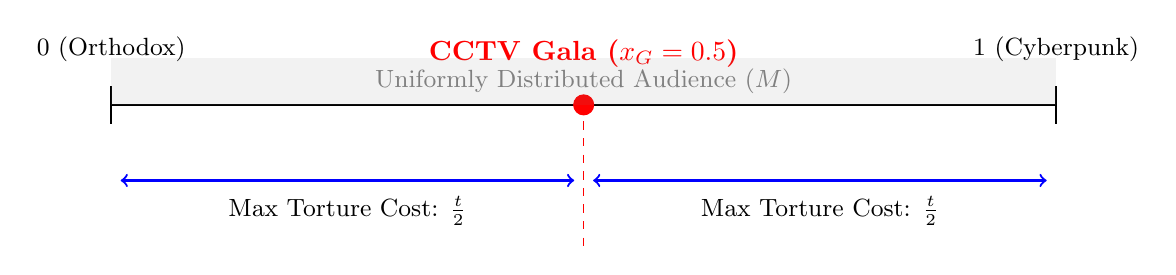
\begin{tikzpicture}[scale=1.2]
    \draw[thick] (0,0) -- (10,0);
    \draw[thick] (0,-0.2) -- (0,0.2) node[above=5pt, font=\small] {$0$ (Orthodox)};
    \draw[thick] (10,-0.2) -- (10,0.2) node[above=5pt, font=\small] {$1$ (Cyberpunk)};
    
    \filldraw[red] (5,0) circle (3pt);
    \node[red, above=10pt, font=\bfseries] at (5,0) {CCTV Gala ($x_G = 0.5$)};
    \draw[dashed, red] (5,0) -- (5,-1.5);
    
    \fill[gray, opacity=0.1] (0,0) rectangle (10,0.5);
    \node[gray, font=\small] at (5, 0.25) {Uniformly Distributed Audience ($M$)};

    \draw[<->, thick, blue] (0.1, -0.8) -- (4.9, -0.8) node[midway, below=2pt, font=\small, text=black] {Max Torture Cost: $\frac{t}{2}$};
    \draw[<->, thick, blue] (5.1, -0.8) -- (9.9, -0.8) node[midway, below=2pt, font=\small, text=black] {Max Torture Cost: $\frac{t}{2}$};
\end{tikzpicture}
\caption{The Frankenstein Equilibrium: Forced Monocentric Supply ($N=1$)}
\begin{figurenotes}[Source]
Author's derivation based on the unwatchability of recent centralized broadcasts.
\end{figurenotes}
\end{figure}

Under this forced monocentricity ($N = 1$), the total social cost spikes to:
\begin{equation}
    TC(1) = F + \frac{M \cdot t}{4}
\end{equation}

Evaluating the socially optimal cost yields $TC(N^*) = \sqrt{M \cdot t \cdot F}$. We define the \textbf{Deadweight Loss (DWL)} as the difference:
\begin{equation}
    DWL = TC(1) - TC(N^*) = F + \frac{M \cdot t}{4} - \sqrt{M \cdot t \cdot F}
\end{equation}

\begin{proposition}
The Deadweight Loss induced by the monocentric Gala is monotonically increasing with respect to the diversity of audience preferences ($\frac{\partial DWL}{\partial t} > 0$).
\end{proposition}

\noindent \textbf{Economic Intuition:} Forcing $N=1$ today is equivalent to compelling $1.4$ billion demographically diverse individuals to wear the exact same ``one-size-fits-all'' sweater. The larger the preference divergence ($t$) becomes, the more suffocating this forced centralization feels, transforming a former Pareto improvement into a massive deadweight loss engine.

\section{Conclusion and Policy Implications}

In this paper, we theoretically demonstrate that the increasing unwatchability of the Spring Festival Gala is a deterministic outcome of economic prosperity and the resulting diversification of consumer preferences. The ``cringe'' factor experienced by modern audiences is not a bug in the directorial process, but a mathematical feature of a forced monopoly operating within an infinite-dimensional aesthetic space.

Our findings suggest that as long as the institutional constraint of $N=1$ remains, the Deadweight Loss will continue to grow monotonically. Therefore, we propose a straightforward, Pareto-improving policy recommendation: \textbf{Aesthetic Decentralization and Broadcasting Deregulation}.

Policymakers should abolish the implicit mandate that forces local and provincial television networks to relay the central broadcast on New Year's Eve. By allowing local networks and digital platforms to host and broadcast their own culturally specific galas simultaneously, the market can naturally transition from the suffocating $N=1$ monopoly to the socially optimal $N^*$. Ultimately, giving the public the freedom to choose their preferred ``dumplings'' is the only sustainable way to maximize national happiness on New Year's Eve.

\FloatBarrier

\begin{thebibliography}{99}

\harvarditem[Dixit and Stiglitz]{Dixit and Stiglitz}{1977}{dixit1977}
Dixit, A. K., and J. E. Stiglitz. (1977). ``Monopolistic Competition and Optimum Product Diversity.'' \textit{The American Economic Review}, 67(3): 297--308.

\harvarditem[Hotelling]{Hotelling}{1929}{hotelling1929}
Hotelling, H. (1929). ``Stability in Competition.'' \textit{The Economic Journal}, 39(153): 41--57.

\harvarditem[Steiner]{Steiner}{1952}{steiner1952}
Steiner, P. O. (1952). ``Program Patterns and Preferences, and the Workability of Competition in Radio Broadcasting.'' \textit{The Quarterly Journal of Economics}, 66(2): 194--223.

\harvarditem[Tiebout]{Tiebout}{1956}{tiebout1956}
Tiebout, C. M. (1956). ``A Pure Theory of Local Expenditures.'' \textit{Journal of Political Economy}, 64(5): 416--424.

\end{thebibliography}

\end{document}